\chapter{Założenia projektowe}
W tym rozdziale został opisany probliem i jego możliwe rozwiązanie.
Została prowadzona wnaliza wymagań: wymagania funkcjonalne i niefunkcjonalne.
W niniejszym rozdiale został przedstawiony początkowy makiet interfejsu użytkownika.

\section{Zarys architektury systemu}
% Описание проблемы:
% Существует проблема найти рабочую станцию зарядки, когда остается мало зарядки в автомобиле.
% Станция может не работать, плохо заряжать, может быть установлена так, что ей невозможно пользоваться, 
% различные сервисы, зачастую, ориентируются на конкретную фигрму заправок и могут не иметь самую актуальную информацию о появлении станций других производителей.
% Хочется просто взять телефон и прямо на карте увидеть где есть станции и посмотреть о ней отзывы реальных людей.

% В результате работы должно быть создано мобильное приложение в которм:
% Водители жлекторомобилей могут легко и быстро находить ближайшие зарядные станции и выбирать лучшую.
% Владельцы стнаций могут добавлять свои станции, что даст им дополнительную рекламу.
% Для определения качества станции должна использоваться система актуальных коментариев и оценок зарегестрированных пользователей.
% Каждый пользователь должен иметь собственный аккаунт для возможности пользоваться приложениемю
% Эта система позволит повысить качество зарядных пунктов.
% Это приложение полнстью поддеживается сообществом: создание и оценка станций производится пользователями.

% В пользовательском интерфейсе, которым я вляется мобильное приложение, должна быть интегрирована карта для упрощения поиска и создания мест.
% Должна быть реализована система регистарции и входа.
% Кроме пользовательского интерфейса долен быть реализована серверная часть, для обработки действий пользователей.
% А также база данных дляхранения станций и коментариев.

% Предположительный макет сервиса:
\paragraph{Opis problemu:}
Istnieje problem ze znalezieniem stacji ładującej samochody elektryczne, gdy w samochodzie pozostaje niewiele ładowania.
Stacja może nie działać, źle ładować, może być zainstalowana tak, że nie można jej używać.
Większość istniejących aplikacji najczęściej mają dostęp tylko do stacji konkretnych firm i mogą nie mieć najbardziej aktualnych informacji o pojawieniu się stacji innych producentów oraz oceny rzeczewistych użytkowników.
Istnieje chęć po prostu wziąć telefon i zobaczyć bezpośrednio na mapie, gdzie są stacje i zobaczyć recenzje prawdziwych ludzi na ten temat..

\paragraph{W wyniku pracy ma powstać aplikacja mobilna w której:}
Kierowcy samochodów elektrycznych mogą łatwo i szybko znaleźć najbliższe stacje ładowania i wybrać najlepszą.
Właściciele stacji mogą dodawać swoje stacje, co da im dodatkową reklamę.
Aby określić jakość stacji, należy użyć systemu aktualnych komentarzy i ocen zarejestrowanych użytkowników.
Każdy użytkownik musi posiadać własne konto, aby móc korzystać z aplikacji.
Taki system może spowodować zwiększenie jakośi punktów ładowania.
Ta aplikacja musi być w pełni wspierana przez społeczność: tworzenie i ocena stacji odbywa się przez użytkowników.

\paragraph{Przypuszczalny układ serwisu:}
Interfejs użytkownika, którym jest aplikacja mobilna, musi mieć zintegrowaną mapę, aby ułatwić wyszukiwanie i tworzenie miejsc.
Należy wdrożyć system rejestracji i logowania.
Oprócz interfejsu użytkownika musi być zaimplementowana część serwerowa do obsługi działań użytkowników.
A także baza danych do przechowywania stacji i komentarzy. Ten układ widać na rysunku \ref{fig:zarysuskladuserwisu}.
\begin{figure}[ht]
    \centering
        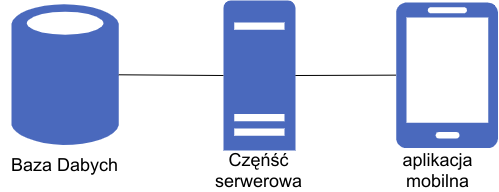
\includegraphics[width=0.4\linewidth]{rys02/uklad_wstepny.png}
        \caption{zarys uskladu serwisu \cite{diagrams_net}}
    \label{fig:zarysuskladuserwisu}
\end{figure}\newline
\newpage
\section{Analiza wymagań}
\subsection{Wymagania funkcjonalne}
W tabeli \ref{tab:wymaganiafunkcjonalne} przedstawione wymagania funkc do aplikacji mobilnej razem z celem ich wdrożenia.
\begin{table}[htb] \small
    \caption{Wymagania funkcjonalne}
    \label{tab:wymaganiafunkcjonalne}
    \begin{tabular}{| m{0.5cm} | m{7cm} | m{7cm} |} 
    \hline
    № & Opis & Cel \\
    \hline
    1 & Użytkownik loguje się do własnego kąta. & Umożliwia korzystanie z funkjalności aplikacji. \\ 
    \hline
    2 & Użytkownik rejestruje się. & Założenie kąta tworzy nowe kąto dla logowania się. \\ 
    \hline
    3 & Użytkownik wyszkuję stacje ładownicze obok wybranego miejca  & dać użytkownikowi możliwość wyboru dogodnej dla niego stacjD \\
    \hline
    4 & Użytkownik ma możliwość określenia własnej pozycji & Robi wyszukiwanie wygodniejszych stacji było bardziej intuicyjne dla użytkownika  \\
    \hline
    5 & Użytkownik ma możliwość przęgliądania mapy razem ze swoją lokalizacją oraz stacji łaowniczych obok wybranego mijsca. & Ułatwienie wyszukiwania najwygodniejszej stacji ładowniczej. \\
    \hline
    6 & Użytkownik ma możliwość wyszukiwania stacji według słów kluczowych & Wyszukiwanie najwygoniejszej stacji z punktu widzenia typu lub nazwy stacji \\
    \hline
    7 & Użytkownik ma możliwość przeglądania informacji dotyczącej stacji ładowniczej, w tym liku oceny i komentarzy innych użytkowników & Podjęcie decyzji i dobór odpowiedniej dla użytkownika stacji \\
    \hline
    8 & Użytkownik ma możliwość wystawienia oceny i napisania komentarzy do wybranej stacji ładowniczej & Określenie jakości stacji. Pozwala na aktualizację danuch dotyczących stacji ladowniczej \\
    \hline
    9 & Użytkownik ma możliwość dowdawania (oznaczenia, tworzenie) nowej stacji & Aktualizacja informacji o dostępnych stacjach \\
    \hline
    10 & Użytkownik, który stworzył stację, ma możliwość zmiany informacji o tej stacji & Aktualizacja informacji istniejącej statji \\
    \hline
\end{tabular}
\end{table}
\newpage
\paragraph{Diagram Przypadków użycia}
Diagram przypadków użycia (rys. \ref{fig:usecasediagram}) graficznie pokazuje użytkowników oraz funkcje aplikacji dostępne do różnych rodzajów użytkowników (w tym przypadku jeden rodzaj).
\begin{figure}[ht]
    \centering
        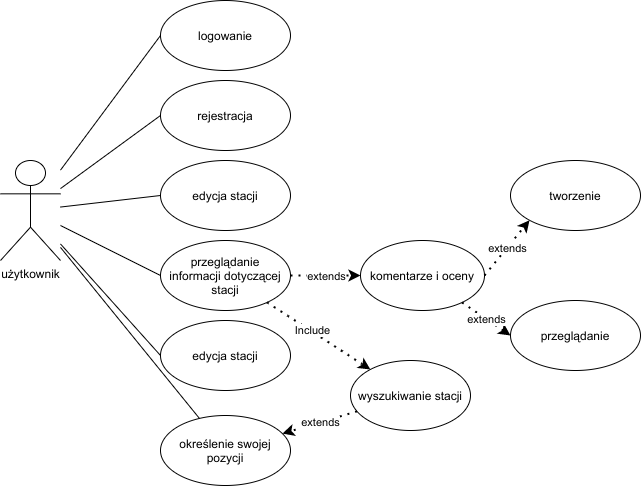
\includegraphics[width=0.7\linewidth]{rys02/use_case_diagram.png}
        \caption{dagram przypadków uzycia \cite{diagrams_net}}
    \label{fig:usecasediagram}
\end{figure}
\newpage
\subsection{Wymagania niefunkcjonalne}
W tabeli \ref{tab:wymaganianiefunkcjonalne} przdstawione wymagania niefunkcjonalne: krótki opis wymagania, typ (jakiej dziedziny to dotyczy) oraz uwagi do tego wymagania.
\begin{table}[htb] \small
    \caption{Wymagania niefunkcjonalne}
    \label{tab:wymaganianiefunkcjonalne}
    \begin{tabular}{| m{0.5cm} | m{3cm} | m{5.75cm} | m{5.75cm} |} 
    \hline
    № & typ & Opis & Uwagi \\
    \hline
    1 & Bezpiczeństwo & Hasła muszą być przechowywane w biezpicznej formie & Hasła nie przchowyją się w pierwotnej formie tylko w formie zaszyfrowanej \\ 
    \hline
    2 & Bezpiczeństwo & Małe ryzyka przechwytywania hasła przaz trzecich osób podczas komunikacji interfejsu użytkownika i części serwerowej & Autentykacja użytkownika na serwerze powinna zachodzić za pomocą tokenów \\ 
    \hline
    3 & Przenoszlność & wdrożenie systemu powinno być szybkie i łatwe & \\ 
    \hline
    4 & Konfigurowalność & Zmiana ustaleń bez konieczosści rekompilacji części serwerowej & zarządzaniem portu na którym działa część serwerowa, wymiana adresu oraz nazwy kolekcji bazy danuch, musi być możliwa za pomocą pliku konfiguracyjnego \\ 
    \hline
    5 & Estetyczne & Przyjazny interfajs użytkownika & Intuicyjny i zrozumiały interfejs \\ 
    \hline
    6 & Ergonomia & Interfejs w języku angielskim & Możliwość kożystania z aplikacji przez dużą libzi \\
    \hline
    7 & Przenoszlność & Aplikacja mobilna musi działać na 90\% telefonów pracujących na systemie Android & Możliwość kożystania z aplikacji przez dużą ilość libzi \\
    \hline
    8 & Estetyczne & kolory muszą być odpowiednio dopasowane & Wykorzystanie małej dopasowanych do sobie ilośći kolorów  \\
    \hline
    9 & Wydajność & Srzybka reakcja systemu & System musi szybko reagować na działania użytkownika \\
    \hline
    10 & Informatywność & System powinien powiadomiać o błędach i sukcesach  & Podczas rażądzania systemem użytkownik powinin zawze wiedzieć jaki wynik jego działania \\
    \hline
    11 & Ergonomia & Wykorzystanie z aplikacji mobilnej za pomocą jednej ręki & Przyciski muszą znajdować się w dolnej części ekranu lub znajdować się w dostępnym miejscu \\
    \hline
    12 & Estetyczne & Wszystkie elementy muszą być w jednym stylu & Niedopuszczalne jest użycie różnych czcionek oraz ciągłej zmiany kolorów \\
    \hline
    13 & Dostęp & Część serwerowa zrobiona zgodnie z regułami Rest (ang. \textit{Representational State Transfer}) API (ang. \textit{Application Programming Interface}) & Przestrzeganie się Best Prakties Rest API \cite{rest_api_best}) \\
    \hline
    14 & Ergonomia & Dla realizacji mapy wykorzystuję się Google Maps[index] & Ułatwia rozumienie interfejsu dla użytkowników \\
    \hline
\end{tabular}
\end{table}
\newpage
\subsubsection{Nażędzia i technologie}
Jako Baza danych wykorzystuje się NoSQL (ang. (ang. \textit{Not only Structured Query Language}) baza danych Mongodb \cite{mongodb,mongodb_doc}.
Część serwerowa napisana w języku Go \cite{golang1,golang2,golang3,godoc} w architekturze Rest API \cite{rest_api_best}.
Część serwerowa i Baza Danych muszą uruchamiać się w Docker kontenerze \cite{docker,docker_doc}.
Aplikacja mobilna działa w systemie Android za pomocą Android Studio \cite{android_doc,android_studio,gradle,gradle_android_doc} w języku Java \cite{java_doc}.
Dla realizacji Google Maps w aplikacji mobilnej wykorzystuję się serwis Google Cloud \cite{google_cloud} Maps SDK for Android (ang. \textit{Maps Software development kit for Android}) \cite{maps_sdk}.

\subsection{Makiety interfejsu użytkownika}
Po analizie wymagań zostały stworzone możliwe makiety aplikacji, która ma powstać.

Na dole ekranu aplikacji znajduje się główne menu zawierające 4 pozycje: mapę, wyszukiwanie stacji, tworzenie stacji i parametry.
Na rysunku \ref{fig:search_makiet} przedstawiony pierwszy etap wyszukiwania stacji ładowania.
Pod polem wyszukiwania znajduje się rozwijane menu, które pozwala wybierać typ wyszukiwania, w tym wyszukiwanie na podstawie pozycji użytkownika oraz nazwy i opisu stacji.
Poniżej znajduje się możliwość do zmiany dystansu wyszukiwania oraz przycisk wyszukiwania.
\begin{figure}[ht]
    \centering
        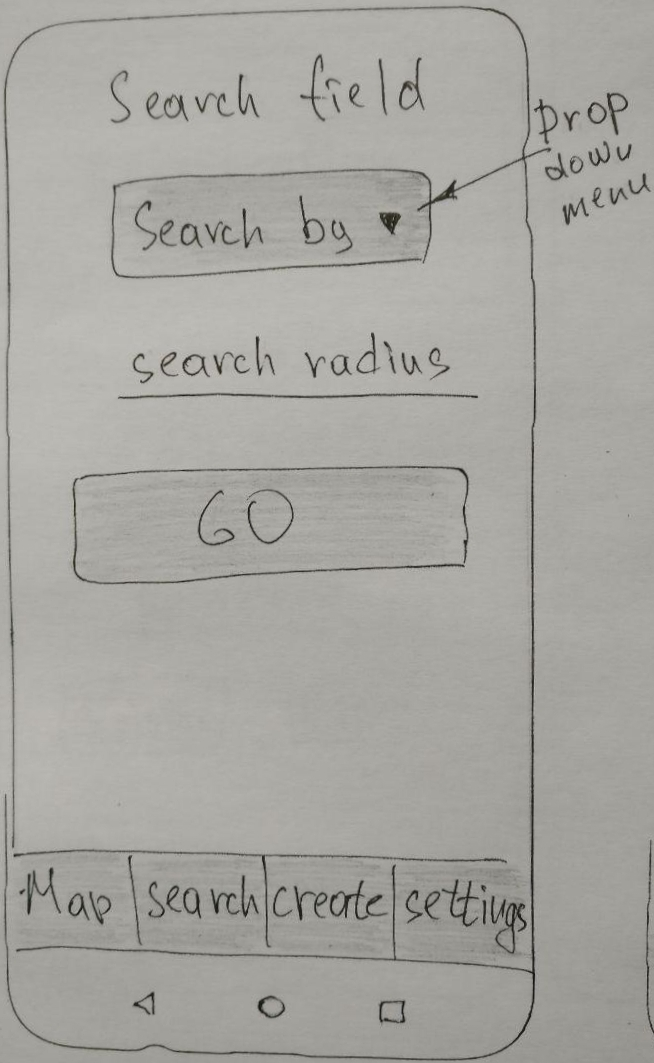
\includegraphics[width=0.4\linewidth]{rys02/search_makiet.jpg}
        \caption{dagram przypadków uzycia}
    \label{fig:search_makiet}
\end{figure}
\newpage
Na tym makiecie (rys. \ref{fig:main_makiet}) został przedstawiony przykładowy sposób wyboru stacji ładowania. Stacje poznaczone markierami na mapie. Dla otrzymania informacji o wybranej stacji (wybierany jest markier na mapie) oraz wyświetlania pozycji użytkownika wykorzystują się okrągłe przyciski z lewej strony ekranu.
\begin{figure}[ht]
    \centering
        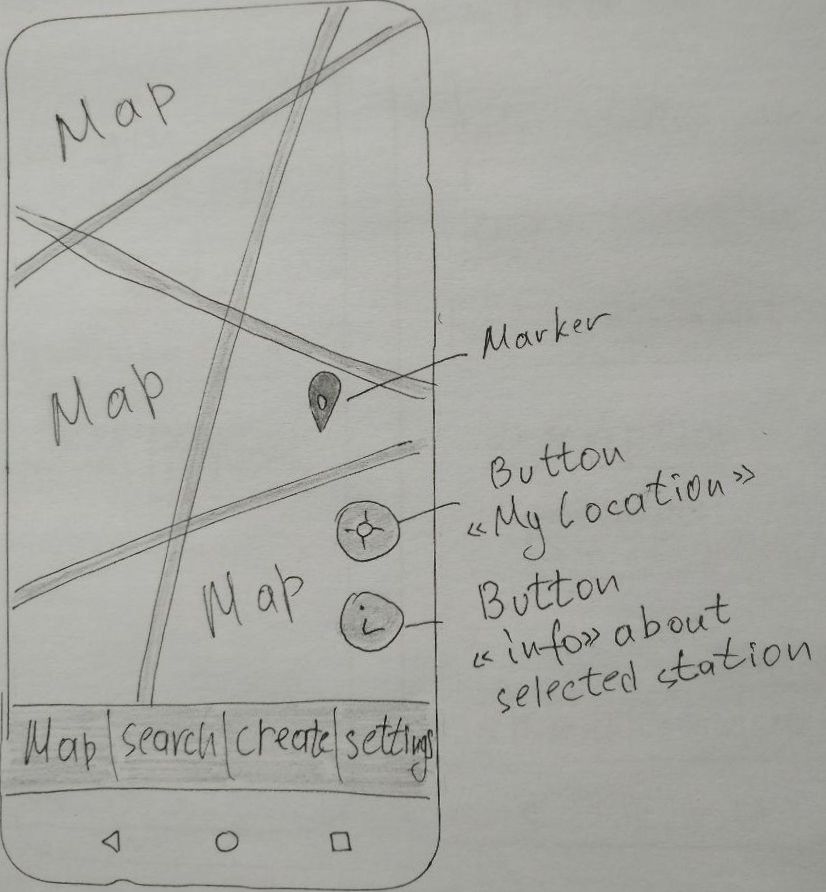
\includegraphics[width=0.5\linewidth]{rys02/main_makiet.jpg}
        \caption{dagram przypadków uzycia}
    \label{fig:main_makiet}
\end{figure}
% \newpage

Podczs tworzenia stacji ładowania (rys. \ref{fig:create_makiet}) dla wygody użytkowania można wybrać miejsce na mapie poprzez odpowiedni przycisk.
\begin{figure}[ht]
    \centering
        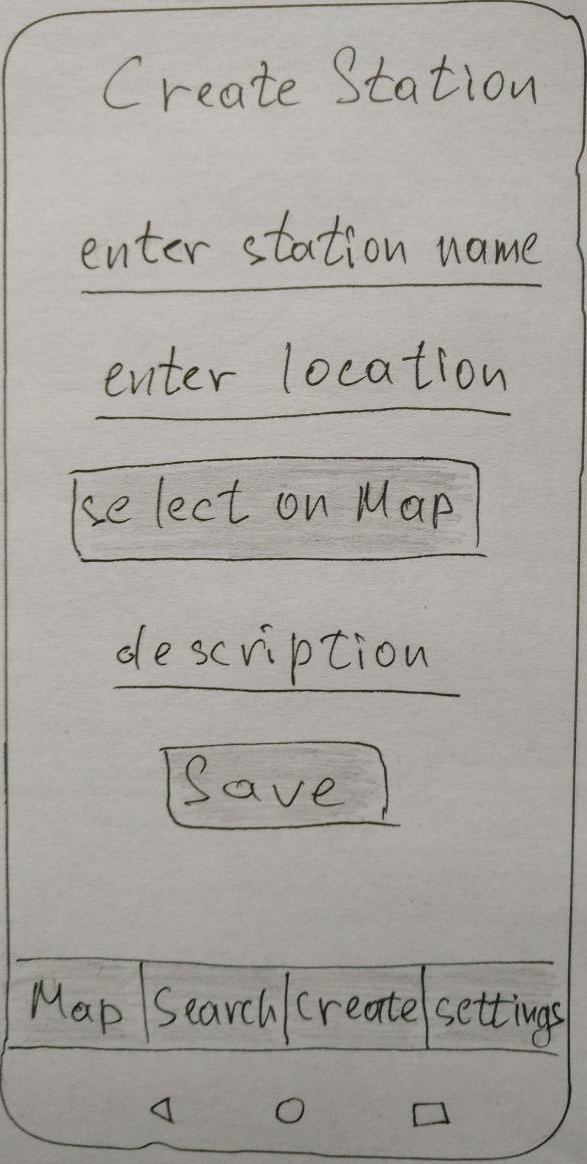
\includegraphics[width=0.3\linewidth]{rys02/create_makiet.jpg}
        \caption{dagram przypadków uzycia}
    \label{fig:create_makiet}
\end{figure}
\newpage
Dla rejestracji i logowania wykorzystują się dwa różne ekrany (rys.\ref{fig:login_makiet} oraz \ref{fig:register_makiet})
\begin{figure}[ht]
    \centering
        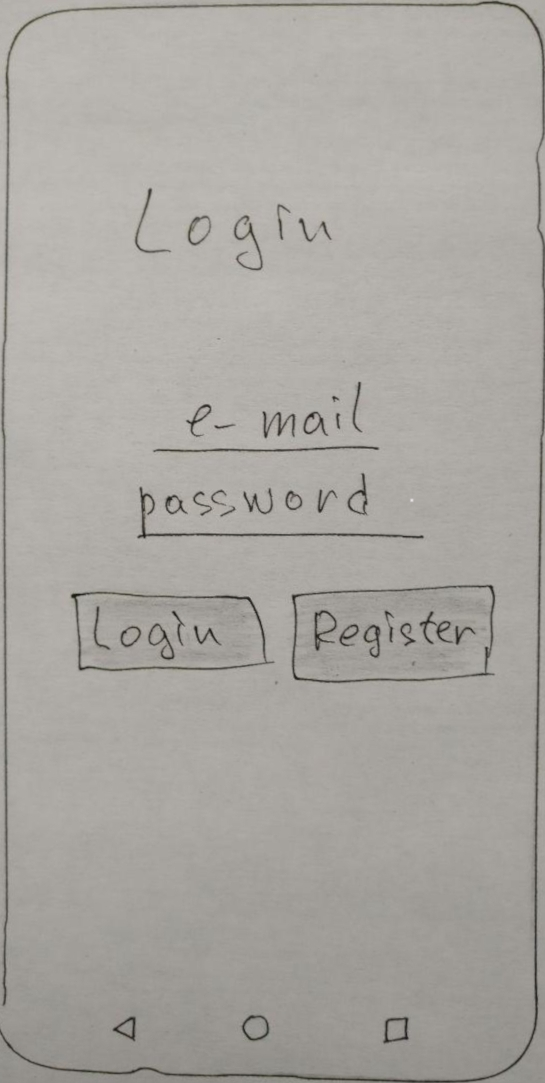
\includegraphics[width=0.3\linewidth]{rys02/login_makiet.jpg}
        \caption{dagram przypadków uzycia}
    \label{fig:login_makiet}
\end{figure}
\begin{figure}[ht]
    \centering
        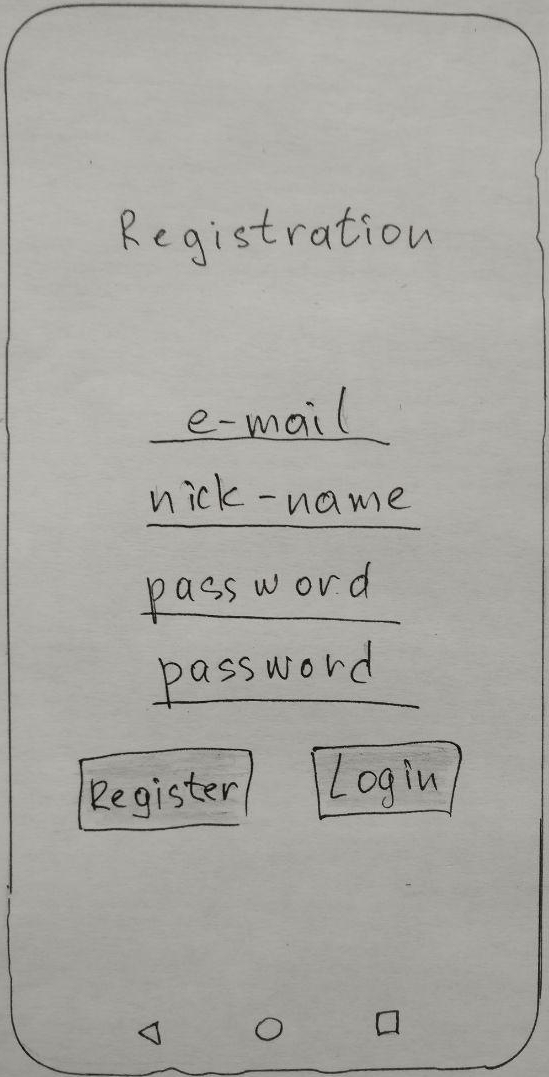
\includegraphics[width=0.3\linewidth]{rys02/register_makiet.jpg}
        \caption{dagram przypadków uzycia}
    \label{fig:register_makiet}
\end{figure}
\newpage


% \paragraph{Część serwerowa:}
% \begin{itemize}
%     \item Visual Studio Code
%     \item Go
%     \item Mongodb
%     \item Redis
%     \item Docker ?
%     \item Docker-compose ?
%     \item Go Modules
%     \item gorilla/mux
%     \item sirupsen/logrus
%     \item mongo-driver
%     \item go-redis/redis
%     \item go-ozzo/ozzo-validation
%     \item yaml.v2
%     \item google/uuid
% \end{itemize}

% \paragraph{Aplikacja mobilna:}
% \begin{itemize}
%     \item Android Studio
%     \item Java   
%     \item ? gradle ?
%     \item RxJava
%     \item OkHttp 3
%     \item Retrofit 2
%     \item Maps SDK for Android
%     \item Google Play services APIs
%     \item gson
% \end{itemize}

% \paragraph{Testowanie: ??}
% \begin{itemize}
%     \item Postman
%     \item Mongodb Compass
%     \item stretchr/testify ??
% \end{itemize}


% \paragraph{Paragraf}
% Tekst\newline
% Tekst
